\documentclass[12pt]{article}
\linespread{1.2}
\usepackage[margin=2cm]{geometry}
\usepackage[utf8]{inputenc}
\usepackage{amsfonts}
\usepackage{amsmath}
\usepackage{multicol}
\usepackage{amsthm}
\usepackage{amssymb,scrextend}
\usepackage{graphicx,tikz, pgfplots}
\usetikzlibrary{arrows}
\pgfplotsset{compat=1.18}
\newtheorem{dfn}{Definition}
\renewcommand{\qed}{\hfill$\blacksquare$}
\let\newproof\proof
\renewenvironment{proof}{\vspace{1em}\begin{addmargin}[2em]{0em}\begin{newproof}}{\end{newproof}\end{addmargin}\qed}
\newenvironment{theorem}[2][Theorem]{\begin{trivlist}
\item[\hskip \labelsep {\bfseries #1} \hskip \labelsep {\bfseries #2.}]}{\end{trivlist}}
\newenvironment{example}[2][Example]{\begin{trivlist}
\item[\hskip \labelsep {\bfseries #1} \hskip \labelsep {\bfseries #2.}]}{\end{trivlist}}
\newenvironment{lemma}[2][Lemma]{\begin{trivlist}
\item[\hskip \labelsep {\bfseries #1} \hskip \labelsep {\bfseries #2.}]}{\end{trivlist}}
\newenvironment{exercise}[2][Exercise]{\begin{trivlist}
\item[\hskip \labelsep {\bfseries #1} \hskip \labelsep {\bfseries #2.}]}{\end{trivlist}}
\newenvironment{problem}[2][Problem]{\begin{trivlist}
\item[\hskip \labelsep {\bfseries #1} \hskip \labelsep {\bfseries #2.}]}{\end{trivlist}}
\newenvironment{corollary}[2][Corollary]{\begin{trivlist}
\item[\hskip \labelsep {\bfseries #1} \hskip \labelsep {\bfseries #2.}]}{\end{trivlist}}
\usepackage{fancyhdr,enumitem,changepage,url}
\pagestyle{fancy}
\author{Warren Atkison}
\date{\today}
\setlength{\headheight}{15pt}
\begin{document}
\fancyhf{}
\fancyhead[L]{Warren Atkison}
\fancyhead[C]{Homework Set 2}
\fancyhead[R]{\today}
\fancyfoot[R]{\thepage}

\section*{Chapter 4}

\begin{exercise}{1} Use graphical analysis to describe the fate of all orbits for each of the following functions. Use different colors for orbits that behave differently
\end{exercise}
\begin{itemize}
	\item[f.] $F(x) = x^2 - x$ (fixed points at $x_0 = 0$ and $x_0 = 2$)
		\begin{center}
			\includegraphics[scale=0.23]{Fig1.4.1f.jpg}
		\end{center}
		If $x_0 < -1$, $F(x)$ goes to infinity. If $x_0 = -1$, $F(x)$ is eventually fixed. If $-1 < x_0 < 0$, $F(x)$ converges to 0. If $0 < x < 2$, then $F(x)$ converges to 0, and if $x > 2$, $F(x)$ goes to infinity.
	\item[g.] $F(x) = \sin x$ (fixed point at $x_0 = 0$)
		\begin{center}
			\includegraphics[scale=0.23]{Fig1.4.1g.jpg}
		\end{center}
		If $x_0 < 0$, then $F(x)$ converges to 0, and if $x_0 > 0$, $F(x)$ also converges to 0.
\end{itemize}
\begin{exercise}{2} Use graphical analysis to find $\{x_0 ~|~ F^{n}(x_0) \to \infty\}$ for each of the following functions	
\end{exercise}
\begin{itemize}
	\item[a.] $F(x) = 2x(1-x)$
		\begin{center}
			\includegraphics[scale=0.23]{Fig1.4.2a.jpg}
		\end{center}
		When $x_0 > 1$ or $x_0 > 1$, then $F^n(x_0) \to -\infty$. There is no $x_0$ s.t. $F^n(x_0) \to +\infty$.
\end{itemize}
\begin{exercise}{3} Sketch the phase portraits for each of the functions in exercise 1.
	\begin{itemize}
		\item[f.] $F(x) = x^2 - x$
			\begin{center}
				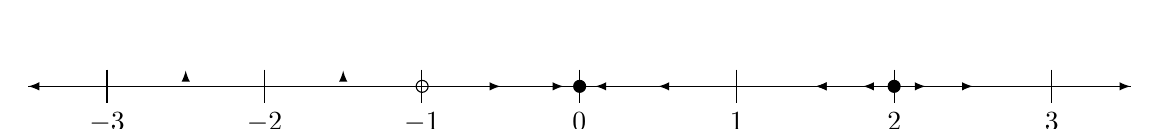
\begin{tikzpicture}[scale = 2]
					\draw[latex-] (-3.5,0) -- (3.5,0) ;
					\draw[-latex] (-3.5,0) -- (3.5,0) ;
					\foreach \x in  {-3,-2,-1,0,1,2,3}
					\draw[shift={(\x,0)},color=black] (0pt,3pt) -- (0pt,-3pt);
					\foreach \x in {-3,-2,-1,0,1,2,3}
					\draw[shift={(\x,0)},color=black] (0pt,0pt) -- (0pt,-3pt) node[below] 
					{$\x$};
					\draw[*-] (2.04,0) -- (2,0) ;
					\draw[*-] (-0.04,0) -- (1,0);
					\draw[latex-] (0.1,0) -- (1,0);
					\draw[latex-] (-0.1,0) -- (-2,0);
					\draw[latex-] (-0.5,0) -- (-2,0);
					\draw[latex-] (-1.5,.1);
					\draw[latex-] (-2.5,.1);
					\draw[latex-] (0.5,0) -- (2,0);	
					\draw[latex-] (1.5,0) -- (2,0);
					\draw[latex-] (1.8,0) -- (3,0);
					\draw[latex-] (2.2,0) -- (2,0);
					\draw[latex-] (1.5,0) -- (2,0);
					\draw[o-] (-1.04,0) -- (2,0);
					\draw[latex-] (2.5,0) -- (1,0);
				\end{tikzpicture}
			\end{center}
		\item[g.] $F(x) = \sin x$
			\begin{center}
				\begin{tikzpicture}[scale = 2]
					\draw[latex-] (-3.5,0) -- (3.5,0) ;
					\draw[-latex] (-3.5,0) -- (3.5,0) ;
					\foreach \x in  {-3,-2,-1,0,1,2,3}
					\draw[shift={(\x,0)},color=black] (0pt,3pt) -- (0pt,-3pt);
					\foreach \x in {-3,-2,-1,0,1,2,3}
					\draw[shift={(\x,0)},color=black] (0pt,0pt) -- (0pt,-3pt) node[below] 
					{$\x$};
					\draw[*-] (-0.04,0) -- (1,0);
					\draw[latex-] (0.45,0) -- (1,0);
					\draw[latex-] (1.45,0) -- (2,0);
					\draw[latex-] (2.45,0) -- (3,0);
					\draw[latex-] (-0.45,0) -- (-1,0);
					\draw[latex-] (-1.45,0) -- (-2,0);
					\draw[latex-] (-2.45,0) -- (-3,0);
				\end{tikzpicture}
			\end{center}
	\end{itemize}
\end{exercise}	

\section*{Chapter 5}
\subsection*{Experiment: Rates of Convergence}
For each function listed below, find the fixed poit $p$, $|F^{'}(p)|$, whether or not $p$ is attracting or neutral, The number of iterations necessary for the orbit of 0.2 to ``reach" $p$, (within $10^{-5}$)
\begin{itemize}
	\item[a.] $F(x) = x^2 + 0.25$ \\
		$p = 1/2$, $|F^{'}(p)| = 1$, $p$ is neutral, 99987 iterations.
	\item[b.] $F(x) = x^2$ \\
		$p = 0$, $|F^{'}(p)| = 0$, $p$ is attracting, 3 iterations. 
	\item[c.] $F(x) = x^2 - 0.24$ \\
		$p = -1/5$, $|F^{'}(p)| = 0.4$, $p$ is attracting, 1 iteration.
	\item[d.] $F(x) = x^2 - 0.75$ \\
		$p = -1/2$, $|F^{'}(p)| = 1$, $p$ is neutral, $> 500000$ iterations.
\end{itemize}
When $|F^{'}(p)| = 1$, there is a really slow rate of convergence, and when $|F^{'}(p)|$ is close to 0, there is a much faster convergence. (c) had the fastest convergence, even though it didn't have the smallest $|F^{'}(p)|$. (d) had the slowest convergence by far, and $p$ was a neutral point in that case. 

\begin{exercise}{1} 
	For each of the following functions, find all the fixed points and classify them as attracting, repelling, or neutral.
	\begin{itemize}
		\item[a.] $F(x) = x^2 - x/2$
			\begin{align*}
				x^2 - x/2 &= x \\ 
				x^2 - 3x/2 &= 0 \\
				x(x - 3/2) &=0
			\end{align*}
			Fixed points occur at $x = 0$ and $x = 3/2$.
			\begin{align*}
				|F^{'}(0)| &= |2(0) - 1/2| & |F^{'}(3/2)| &= |2(3/2) - 1/2| \\
					   &= |-1/2| & 			  &= |3 - 1/2| \\
					   &= 1/2 & 			  &= 5/2
			\end{align*}
			The fixed point $x = 0$ is attracting and the fixed point $x = 5/2$ is repelling.
		\item[c.] $F(x) = 3x(1 - x)$
			\begin{align*}
				3x - 3x^2 &= x \\
				-3x^2 + 2x &= 0 \\
				x(-3x + 2) &= 0
			\end{align*}
			Fixed points occur at $x = 0$ and $x = 2/3$.
			\begin{align*}
				|F^{'}(0)| &= |3 - 6(0)| & |F^{'}(2/3)| &= |3 - 6(2/3)| \\
					   &= 3 & 			&= |3 - 4| \\
					   && 				&= 1
			\end{align*}
			The fixed point $x = 0$ is repelling and the fixed point $x = 2/3$ is neutral.
	\end{itemize}
\end{exercise}

\begin{exercise}{2} For each of the following functions, zero lies on a periodic orbit. Classify this orbit as attracting, repelling, or neutral.
	
\end{exercise}
\begin{itemize}
	\item[d.] $F(x) = |x - 2| - 1$
		\[
			\{0,1,0,1, \ldots \}
		\]
		0 lies on period 2 orbit.
		\begin{align*}
			|(F^{2})^{'}(0)| &= |F^{'}(1)|\cdot|F^{'}(0)| \\
				       &= 1
		\end{align*}
		This orbit is neutral.
\end{itemize}
\begin{exercise}{3}
	Suppose $x_{0}$ lies on a cycle of prime period $n$ for the doubling function $D$. Evaluate $(D^n)^{'}(x_0)$. Is this cycle attracting or repelling?
\end{exercise}
Let $\{x_0,x_1,\ldots,x_{n-1}\}$ be the cycle containing $x_0$.
\begin{align*}
	(D^{n})^{'}(x_0) &= D^{'}(x_{n-1}) \cdot D^{'}(x_{n-2}) \cdot \ldots \cdot D^{'}(x_0) \\
			 &= 2^n
\end{align*}
This cycle is repelling.

\begin{exercise}{4}
	Each of the following functions has a neutral fixed point. Find this fixed point and, using graphical analysis with an accurate graph, determine if it is weakly attracting, weakly repelling, or neither.
	\begin{itemize}
		\item[a.] $F(x) = x + x^2$
			\begin{align*}
				x + x^2 &= x \\
				x^2 &= 0 \\
				x &= 0
			\end{align*}	
			$x = 0$ is our neutral fixed point.
			\begin{center}
				\includegraphics[scale = 0.23]{Fig2.5.4a.jpg}
			\end{center}
	\end{itemize}
	$x_0 = 0$ is weakly attracting on the interval $-1 < x < 0$, and weakly repelling everywher else besides the fixed point $x = 0$ and $x = -1$ which is eventually fixed.
\end{exercise}

\end{document}
